\documentclass[a4paper,10pt]{article}

%% Paquetes Adicionales %%

\usepackage[spanish]{babel}
\selectlanguage{spanish}
\spanishdecimal{.}
\addto\captionsspanish{\def\tablename{Cuadro}}
\usepackage{fancyhdr}
\usepackage{graphics}
\usepackage[dvips]{graphicx}
\usepackage[normal]{caption2}
\usepackage{amsfonts,amssymb,amsmath,amsthm}
\usepackage[T1]{fontenc}
\usepackage{moreverb}

%% Declaracion de comandos %%

\newtheorem{lema}{Lema}
\newtheorem{teor}{Teorema}
\newtheorem{propos}{Proposici\'on}
\newtheorem{corol}{Corolario}

\newcommand{\mivec}[1]{\mathbf{#1}}
\newcommand{\vers}[1]{\mivec{\check{#1}}}
\newcommand{\deriv}[2]{\frac{\mathrm{d}#1}{\mathrm{d}#2}}
\newcommand{\expo}[1]{~10^{#1}}
\newcommand{\uni}[1]{\mathrm{#1}} 

\newcommand{\prop}[1]{\begin{propos} #1 \end{propos}}
\newcommand{\teo}[1]{\begin{teor} #1 \end{teor}}
\newcommand{\cor}[1]{\begin{corol} #1 \end{corol}}
\newcommand{\lem}[1]{\begin{lema} #1 \end{lema}}

%% Encabezado y Pie de Pagina %%

\pagestyle{plain}
\lhead{}
\chead{}
\rhead{}
\cfoot{\thepage}
\renewcommand{\footrulewidth}{0.4pt}

\makeindex

%% Titulo %%
\begin{document}
\title{{Computaci\'on Gr\'afica \\ Trabajo pr\'actico especial 1 - Ray Caster\\ Grupo 2}}
\author{Guillermo Campelo\\Juan Ignacio Go\~ni\\Juan Tenaillon\\Santiago Vazquez}
\date{}

%% Comienzo del documento %%

\maketitle

\begin{abstract}

Se dise\~n\'o y desarroll\'o un motor de Ray Casting, determinando intersecciones entre rayos originados en la c\'amara y objetos.
Esto permite representar escenas con figuras dentro.

\textbf{Palabras Clave: }\emph{Ray Casting, escena, rayos, objetos, primitivas, tri\'angulo, esfera, cuadril\'atero.}.
\end{abstract}

%\thispagestyle{fancy}

%% COMIENZO DEL TEXTO %%
\section{Introducci\'on}
\label{introduccion}

En este informe, se explicar\'a el dise\~no y el desarrollo del motor de Ray Casting, explicando cada una de sus componentes y que nos motivo a desarrollarlas de la manera en que lo hicimos.

En la segunda secci\'on nos enfocaremos en el motor de Ray Casting y como se utiliza, luego en la tercera secci\'on nos enfocaremos en la escena y los objetos que la componen, como sean las esferas, 
los tri\'angulos y los cuadril\'ateros.  En la cuarta secci\'on nos enfocaremos en los resultados obtenidos y por \'ultimo, en la quinta secci\'on, presentamos nuestras conclusiones.
\section{Ray Caster}
\label{raycaster}

\subsection{Descripci\'on}
\label{subseccion}
Ray Casting es una t\'ecnica que utiliza la intersecci\'on de rayos con una superficie para resolver un conjunto de problemas en el campo de la computaci\'on gr\'afica.  Representa una soluci\'on f\'acil al problema de la representaci\'on en una escena.

En este caso se modela una escena almancenada en memoria, para la cual se fija una posici\'on y direcci\'on para la c\'amara.  Desde esta se disparan rayos a intervalos regulares y para cada uno se muestra el color correspondiente al objeto m\'as cercano con el que colisiona.

\subsection{La Escena}

Actualmente existen $6$ escena predefinidas, pero la arquitectura contempla obtener nuevas escenas desde otras fuentes, por ejemplo de
un archivo. En la secci\'on \ref{escenas} se describen y se muestran las im\'agenes obtenidas.

\subsection{La C\'amara}

El modelo de la c\'amara contempla el \'angulo de apertura del lente para el c\'alculo de la representaci\'on de la escena.
Conociendo el \'angulo de apertura horizontal y la relaci\'on entre el ancho y el alto de la imagen, se toma un plano imaginario
con normal al vector director de la c\'amara. Se utiliza un vector para dar la rotaci\'on de la c\'amara y se realizan las correcciones
necesarias al plano.

Luego en funci\'on de la resoluci\'on horizontal y vertical, se toma el delta \'angulo en el eje $x$ y eje $y$ relativos a la c\'amara.

El Ray Caster iterar\'a por los pixeles de la imagen y la c\'amara devolver\'a el rayo con origen en el centro de la c\'amara y que
pase por el correspondiente pixel.

\subsection{Modo de Uso}
Para ejecutar el Ray Caster hay diferentes opciones.  A continuaci\'on especificamos cuales son estas opciones y mostramos su modo de uso.

\subsubsection{Nombre de Archivo de Entrada}
Para poder utilizar el Ray Caster, es necesario especificar un nombre de archivo de entrada.  Los posibles nombres para las escenas de entradas son de la forma $scene\#.sc$ y para utilizar el ray caster con un archivo de este tipo hay que especificarlo de la siguiente manera:

\begin{center}
 \textbf{\texttt{-i [nombre de archivo]}}
\end{center}

Suponiendo un nombre de escena $scene1.sc$, una posible llamada al Ray Caster ser\'ia:

\begin{center}
 \textbf{\texttt{cg\_tpe1 -i scene1.sc}}
\end{center}

Este campo es \textbf{obligatorio} para poder utilizar la aplicaci\'on.
\subsubsection{Nombre de Archivo de Salida}

Al ejecutar el Ray Caster, se producir\'a un archivo de salida.  El usuario de la aplicaci\'on puede elegir un nombre en particular para el mismo.  Esto se hace utilizando la siguiente opci\'on:

\begin{center}
  \textbf{\texttt{-o [nombre de archivo]}}
\end{center}

En caso de no especificar ning\'un nombre en particular para el mismo, el nombre del archivo de salida ser\'a el mismo que el archivo de entrada pero con extensi\'on $*.bmp$ o $*.png$.  Suponiendo que se requiere un nombre de archivo espec\'ifico, el uso de la opci\'on es la siguiente:

 \begin{center}
 \textbf{\texttt{cg\_tpe1 -i scene1.sc -o scene1.png}}
\end{center}

El uso de esta opci\'on \textbf{no es obligatoria} para el uso de la aplicaci\'on.

\subsubsection{Pixeles en la Imagen de Salida}
Para indicar la cantidad de pixeles en la imagen de salida, se utiliza la opci\'on indicada a continuaci\'on:

\begin{center}
  \textbf{\texttt{-size <alto>x<ancho>}}
\end{center}

En caso de no especificar ninguna cantidad en particular, se utilizar\'a el tama\~no por defecto de 640x480 pixeles.  Un ejemplo de su uso ser\'ia:

 \begin{center}
 \textbf{\texttt{cg\_tpe1 -i scene1.sc -size 800x600}}
\end{center}

Este campo \textbf{no es obligatorio} para poder utilizar la aplicaci\'on.

\subsubsection{Campo de Visi\'on}
Para indicar el \'angulo de apertura horizontal en grados, se va a utilizar:

\begin{center}
  \textbf{\texttt{-fov x}}
\end{center}

donde x es un n\'umero en grados.  En caso de no especificarse ning\'un \'angulo, el valor por defecto es de 60 grados.  Un ejemplo de su uso ser\'ia:

 \begin{center}
 \textbf{\texttt{cg\_tpe1 -i scene1.sc -fov 80}}
\end{center}

Este campo \textbf{no es obligatorio} para poder utilizar la aplicaci\'on.

\subsubsection{Asignaci\'on de Color}
Para indicar el modo de asignaci\'on de color de las primitivas en la escena, hay que utilizar esta opci\'on:
\begin{center}
  \textbf{\texttt{-cm [random | ordered]}}
\end{center}

Donde $random$ es el valor por defecto e indica una asignaci\'on de colores de forma aleatoria y $ordered$, donde la asignaci\'on de color depender\'a del orden en que fueron descubiertas las primitivas.  El orden de asignaci\'on es: $violeta$, $azul$, $verde$, $amarillo$, $naranja$ y $rojo$. El orden de asignaci\'on a las figuras en la escena esta determinado por la secuencia de colisiones. El primer objeto dibujado en pantalla, obtiene el primer color de la lista. Luego siguen los dem\'as objetos con los siguientes colores.
Un ejemplo de su uso ser\'ia:
 \begin{center}
 \textbf{\texttt{cg\_tpe1 -i scene1.sc -cm ordered}}
\end{center}

El uso de esta opci\'on \textbf{no es obligatoria} para el uso de la aplicaci\'on.

\subsubsection{Variaci\'on del Color}

Para indicar el modo de variaci\'on del color de los elementos de la escena, hay que utilizar esta opci\'on:

\begin{center}
  \textbf{\texttt{-cv [linear | log]}}
\end{center}

Donde $linear$ es el valor por defecto e indica que la variaci\'on del color es proporcional a la distancia entre el punto de colisi\'on en la primitiva y la posici\'on de la c\'amara y $log$, donde la variaci\'on del color es logar\'itmica.  Un ejemplo de su uso ser\'ia:

 \begin{center}
 \textbf{\texttt{cg\_tpe1 -i scene1.sc -cv log}}
\end{center}

El uso de esta opci\'on \textbf{no es obligatoria} para el uso de la aplicaci\'on.

\subsubsection{Tiempo de Ejecuci\'on}

Para determinar el tiempo que demor\'o la aplicaci\'on para renderizar la escena indicada, se utiliza:

\begin{center}
  \textbf{\texttt{-time}}
\end{center}

Un ejemplo de su uso ser\'ia:

 \begin{center}
 \textbf{\texttt{cg\_tpe1 -i scene1.sc -time}}
\end{center}
El uso de esta opci\'on \textbf{no es obligatoria} para el uso de la aplicaci\'on.

\section{Primitivas}

Para modelar las escenas, se debieron modelar los distintos objetos presentes en la misma.  En este caso, las primitivas seleccionadas fueron: \emph{tri\'angulo}, \emph{cuadril\'atero} y \emph{esfera}.

A continuaci\'on explicaremos, para cada una de las primitivas, c\'omo se decidi\'o el dise\~no de las mismas.

\subsection{Rayo}

\subsubsection{Representaci\'on}

\subsection{Tri\'angulo}
\label{triangulo}
\subsubsection{Representaci\'on}

\subsubsection{Intersecci\'on}

\subsection{Cuadril\'atero}

\subsubsection{Representaci\'on}
Para representar un cuadril\'atero, se pens\'o en la utilizaci\'on de los cuatro puntos en el espacio.  Se eligi\'o esta representaci\'on debido a que, adem\'as de ser la m\'as simple, tambi\'en resulta \'util al momento de calcular los planos en los que se encuentra para poder determinar la intersecci\'on de los rayos con el mismo.

En la siguiente secci\'on, se explicar\'a a grandes rasgos, c\'omo fue realizada la intersecci\'on del rayo con el cuadril\'atero.
\subsubsection{Intersecci\'on}
Para determinar la intersecci\'on entre un cuadril\'atero y un rayo, se dividi\'o el c\'alculo en dos partes.

La primera parte consistie en determinar si el rayo en cuesti\'on, intersecta al plano que contiene a la primitiva.  Para realizar esto, se calcula el \emph{plano contenedor} y una vez obtenida la ecuaci\'on del tipo

 \begin{center}
 Ax + By + Cz + D = 0
\end{center}

En esta ecuaci\'on, se obtiene el $t$ para el cual el rayo intersecta al plano y en caso de no existir tal $t$, el rayo no intersecta a la primitiva, pero en caso de si existir, es necesario determinar si el punto de intersecci\'on entre el plano y el rayo pertenece a la primitiva.

Para la segunda parte del c\'alculo, se supuso que cualquier cuadril\'atero son dos tri\'angulos.  Donde si el cuadril\'atero tiene por puntos $p1$, $p2$, $p3$ y $p4$, el primer tri\'angulo estar\'ia compuesto por $p1$, $p2$ y $p3$ y el segundo estar\'ia compuesto por $p1$, $p4$ y $p3$.
Asumiendo esto, despues se utiliza una funci\'on que determina si un punto est\'a dentro de un tri\'angulo que fue explicada en la secci\'on \ref{triangulo}.

\subsection{Esfera}

\subsubsection{Representaci\'on}

\subsubsection{Intersecci\'on}

\section{Resultados Obtenidos}
\label{escenas}
El motor de Ray Casting tiene la capacidad de renderizar cualquier escena que est\'e cargada en memoria.  En esta implementaci\'on, se decidi\'o mostrar la capacidad del motor mediante la renderizaci\'on de seis escenas.  Tres de ellas, propuestas por la c\'atedra y las otras tres, propuestas por el grupo desarrollador.  A continuaci\'on, ense\~naremos cada una de ellas con una breve descripci\'on.

\subsection{Primera Escena: \texttt{scene1.sc}}
Esta escena contiene una pir\'amide rectangular, cuyo lado de la base y su altura tiene una longitud de 5.  La base de la misma est\'a centrada en el origen, en su v\'ertice superior tiene posicionada en perfecto equilibrio una esfera de radio 1 y a una distacia de 3, en cada uno de los v\'ertices, tiene una esfera de radio 0.5. Ver \textbf{Figura \ref{fig:1}}.

\begin{figure}[h]
 \centering
 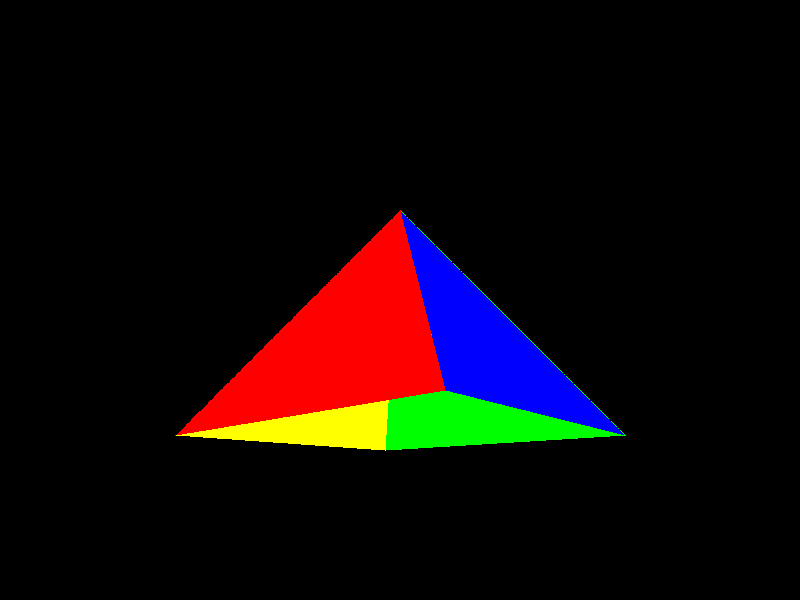
\includegraphics[width=320pt,keepaspectratio=true]{../scene1.png}
 % scene1.png: 640x480 pixel, 72dpi, 22.58x16.93 cm, bb=0 0 640 480
 \caption{Escena n\'umero 1, tri\'angulo y esferas.}
 \label{fig:1}
\end{figure}

\subsection{Segunda Escena: \texttt{scene2.sc}}
Esta escena contiene 64 esferas de radio 0.5 dispuestas en forma de cubo.  Esto es, 4 esferas sobre el eje $x$, 4 sobre el eje $y$ y 4 sobre el eje $z$ formando un cubo de 64 esferas. Cada una de ellas debe estar a una distacia de 1.5 de la otra y el centro de la figura debe estar en el centro del sistema de coordenadas. Ver \textbf{Figura \ref{fig:2}}.

\begin{figure}[h]
 \centering
 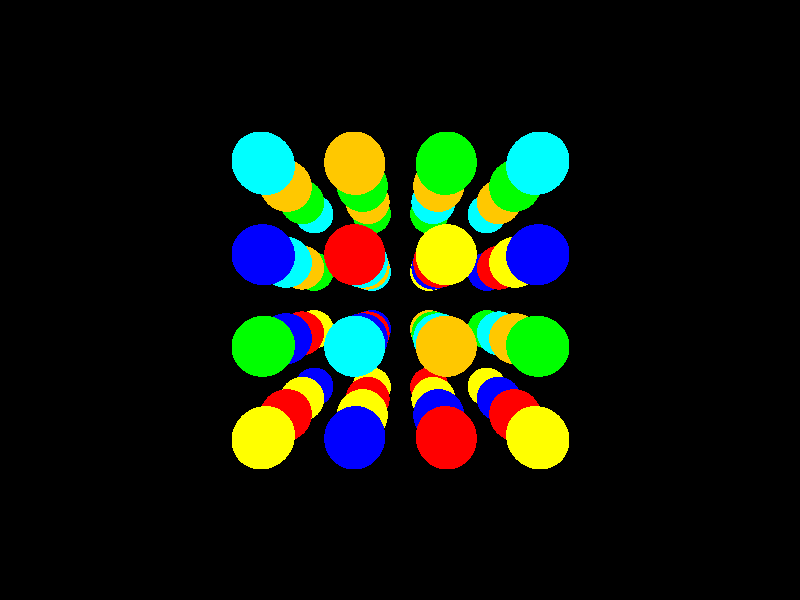
\includegraphics[width=320pt,keepaspectratio=true]{../scene2.png}
 % scene1.png: 640x480 pixel, 72dpi, 22.58x16.93 cm, bb=0 0 640 480
 \caption{Escena n\'umero 2, esferas formando un cubo.}
 \label{fig:2}
\end{figure}

\subsection{Tercera Escena: \texttt{scene3.sc}}
Esta escena contiene, de forma intercalada, 3 cubos de lados 2 y dos esferas de radio 1 alineados de manera centrada sobre el eje $x$.  Las bases de los cubos y las esferas est\'an apoyadas sobre el eje $y=0$ y la separaci\'on entre las figuras es de 0.5. Ver \textbf{Figura \ref{fig:3}}.

\begin{figure}[h]
 \centering
 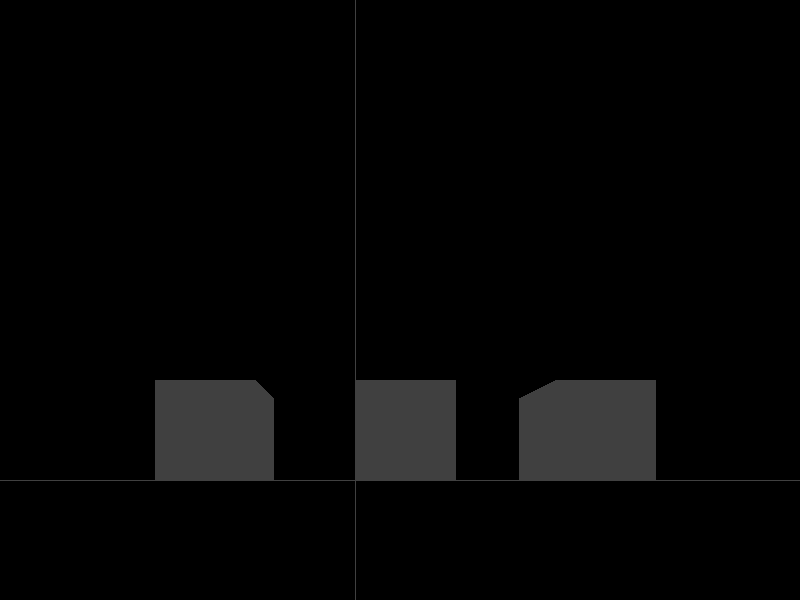
\includegraphics[width=320pt,keepaspectratio=true]{../scene3.png}
 % scene3.png: 800x600 pixel, 72dpi, 28.22x21.17 cm, bb=0 0 800 600
 \caption{Escena n\'umero 3, cubos y esferas intercaladas.}
 \label{fig:3}
\end{figure}

\subsection{Cuarta Escena: \texttt{scene4.sc}}
Esta escena es similar a la tercera escena, pero la distancia entre las primitivas es 0.  Ver \textbf{Figura \ref{fig:4}}.

\begin{figure}[h]
 \centering
 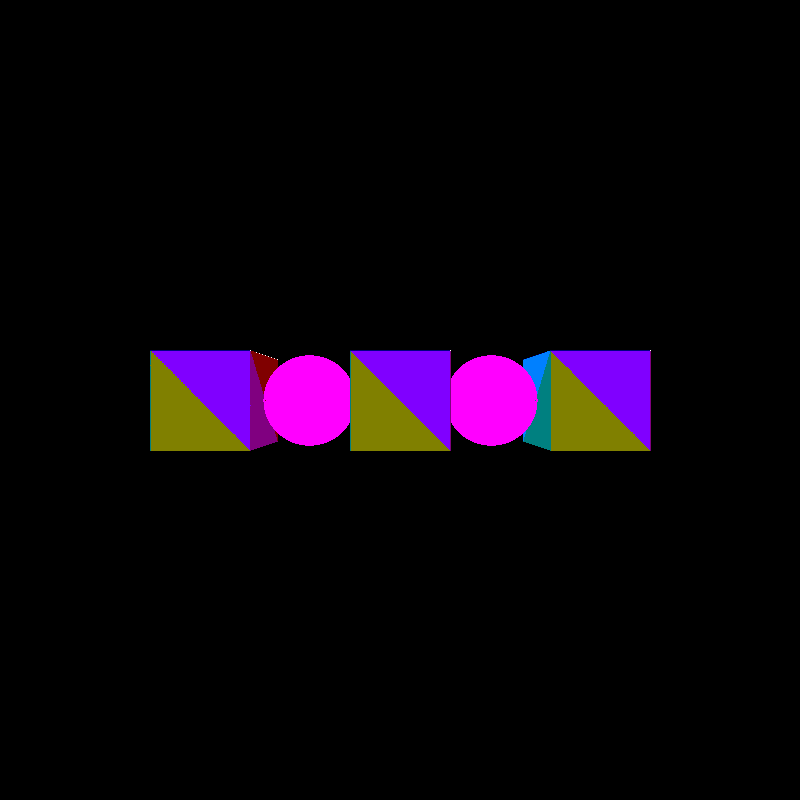
\includegraphics[width=320pt,keepaspectratio=true]{../scene4.png}
 % scene3.png: 800x600 pixel, 72dpi, 28.22x21.17 cm, bb=0 0 800 600
 \caption{Escena n\'umero 4, cubos y esferas intercaladas.}
 \label{fig:4}
\end{figure}

\subsection{Quinta Escena: \texttt{scene5.sc}}
Esta escena contiene 11 esferas alineadas a lo largo del eje $x$.  Todas ellas a una distancia de 0.5 y con un radio de 0.5. Ver \textbf{Figura \ref{fig:5}}.

\begin{figure}[h]
 \centering
 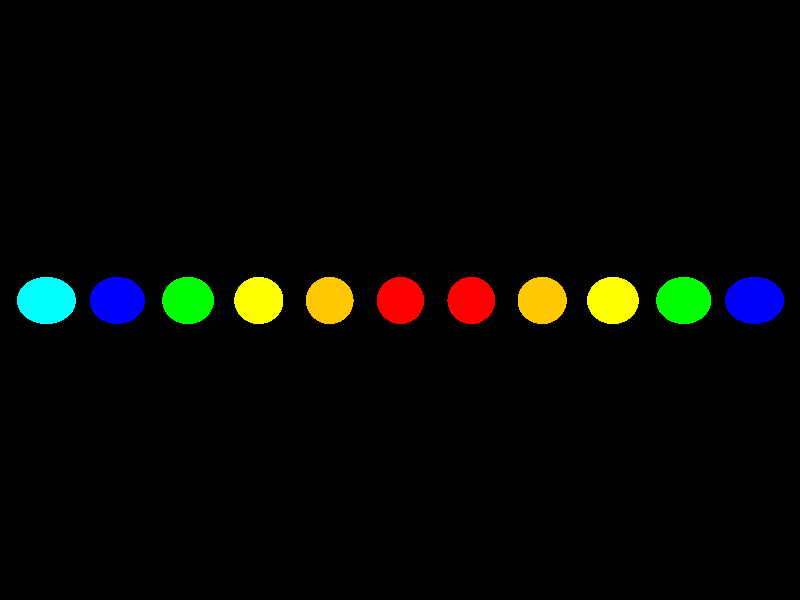
\includegraphics[width=320pt,keepaspectratio=true]{../scene5.png}
 % scene3.png: 800x600 pixel, 72dpi, 28.22x21.17 cm, bb=0 0 800 600
 \caption{Escena n\'umero 5, 11 esferas alineadas.}
 \label{fig:5}
\end{figure}

\subsection{Sexta Escena: \texttt{scene6.sc}}
Esta escena contiene 20 tri\'angulos que forman una estrella con centro en el centro del sistema de coordenadas.  Ver \textbf{Figura \ref{fig:6}}.

\begin{figure}[h]
 \centering
 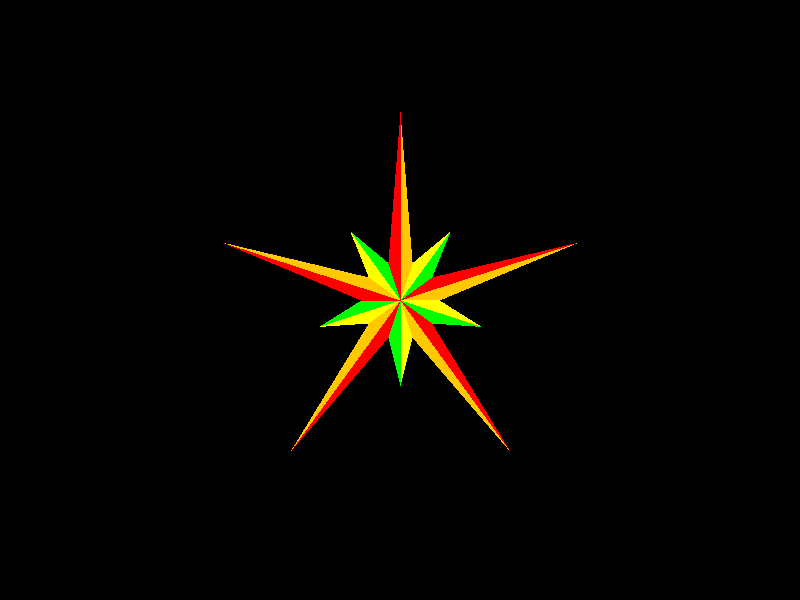
\includegraphics[width=320pt,keepaspectratio=true]{../scene6.png}
 % scene3.png: 800x600 pixel, 72dpi, 28.22x21.17 cm, bb=0 0 800 600
 \caption{Escena n\'umero 6, 20 tri\'angulos formando una estrella.}
 \label{fig:6}
\end{figure}

\section{Comentarios Finales}

\section{Bilbiograf\'ia}
\end{document}